
% C:IKNP03 https://www.iacr.org/archive/crypto2003/27290145/27290145.pdf
% Nie07  "Extending Oblivious Transfers Efficiently How to get Robustness Almost for Free"
% C:KelOrsSch15  https://eprint.iacr.org/2015/546.pdf
% RSA:OrrOrsSch17  https://eprint.iacr.org/2016/933.pdf
% EC:ALSZ15 https://eprint.iacr.org/2015/061.pdf

\newcommand{\rr}{\ensuremath{\boldsymbol{r}}}
\renewcommand{\tt}{\ensuremath{\boldsymbol{t}}}
\newcommand{\ww}{\ensuremath{\boldsymbol{w}}}
\newcommand{\cc}{\ensuremath{\boldsymbol{c}}}
\newcommand{\uu}{\ensuremath{\boldsymbol{u}}}
\newcommand{\qq}{\ensuremath{\boldsymbol{q}}}
\newcommand{\bb}{\ensuremath{\boldsymbol{b}}}
\newcommand{\vv}{\ensuremath{\boldsymbol{v}}}
\newcommand{\nc}{\ensuremath{{n_\mathcal{C}}}}
\newcommand{\kc}{\ensuremath{{k_\mathcal{C}}}}
\newcommand{\dc}{\ensuremath{{d_\mathcal{C}}}}

\section{OT Extension}


In this section we explore the rich implications Endemic OT has on efficient 1-out-of-$N$ OT extension along with presenting two new attacks and fixes of existing OT extension protocols\cite{C:KelOrsSch15, RSA:OrrOrsSch17} with Uniform Message security\footnote{\cite{C:KelOrsSch15, RSA:OrrOrsSch17} refer to uniform OT as random OT $\mathcal{F}^{m,\kappa}_{\textsf{ROT}}$}. These protocols are derived from the seminal black-box protocol of Ishia, Kilian, Nissim and Petrank\cite{C:IKNP03}. We note that in all cases the Sender Chosen Message variant of these protocols\cite{C:IKNP03, C:KelOrsSch15, RSA:OrrOrsSch17} are secure. %In particular, these Sender Chosen Message protocol perform the following transformations $\OOT^\send\overset{\pi_1}{\rightarrow} \OOT^\E \overset{\pi_2}{\rightarrow} \OOT^\send$. However, as we will explore later, \figureref{fig:OTExtrelations} suggestions that a more efficient transformation exists where $\pi_1$ takes $\OOT^\E$ as input, e.g. a two round extension protocol satisfying $\OOT^\rec$.



The functionality of 1-out-of-$N$ OT extension allows $\nc\approx\kappa$ instances of 1-out-of-2 OTs to be transformed into $m=\textsf{poly}(\kappa)$ instances of 1-out-of-$N$ OTs. There are several advantages of this transformation 1) $m$ can be polynomial times larger than $\nc$. 2) Only symmetric key cryptography is required which provides a larger performance improvement. 3) In some cases $N$ can be exponential in the security parameter $\kappa$. The 1-out-of-2 OTs that are being transformed are referred to as \emph{Base OTs}. Existing protocols\cite{C:IKNP03,EC:ALSZ15, C:KelOrsSch15, RSA:OrrOrsSch17} have called for the use of base OTs with the Sender Tweakable Message Security notion, e.g. $\OOT^\send$. However, this requirement can be relaxed to allow the base OTs to only achieve Endemic security. As shown by \figureref{fig:OTExtrelations}, in both cases ($\OOT^\send$ or $\OOT^\E$ base OTs) the OT extension protocol outputs messages that satisfy the Endemic security notion.  Tradition OT extension protocols, e.g. \cite{C:IKNP03,EC:ALSZ15, C:KelOrsSch15}, then apply the $\Pi^{\send}_{1,N}$ transform from \figureref{fig:protoSendOT} to realize the Sender Chosen Message functionality $\OOT^\send$. This observation suggests that more efficient OT extension can be realized by replacing Sender Chosen Message base OTs with Endemic OTs, e.g. our protocol.

In addition, the authors of \cite{C:KelOrsSch15,RSA:OrrOrsSch17} suggest that the $\Pi^{\send}_{1,N}$ transform that was originally specified by \cite{C:IKNP03} can be removed and resulting protocol would satisfy the Uniform Message security notion. However, as previously stated, we show this not to be the case and that the protocol only achieve Endemic security. We note that many protocols that utilize Uniform Message security can likely tolerate the weaker notion of Endemic security, e.g. \cite{EC:RinRos17,CCS:RinRos17}.  However, other protocols such as the set inclusion protocol of \cite[Figure 5]{RSA:OrrOrsSch17} are insecure\footnote{The sender set all the OT messages to be the same value and force the receiver to conclude their item is in the sender's set.} when Uniform Message security is not satisfied. 

Uniform Message security can be achieved in several ways. One solution is the the black-box transformation $\Pi^\U_{1,N}$ of \figureref{fig:uniformOT} which lifts an OT protocol with Endemic security to satisfy Uniform Message security. However, this would require additional rounds and significant communication. We demonstrate an alternative solution which replaces the base OTs with a protocol that satisfies Uniform Message, Uniform Selection security $\OOT^{\U u}$ and prove that this yields an OT extension protocol with Uniform Message security without the need to modify the extension protocol. More generally, \figureref{fig:OTExtrelations} shows the relation between different base OT security notions and the resulting OT extension message security. For example, the protocols of \cite{C:IKNP03,EC:ALSZ15, C:KelOrsSch15} perform
$$
\OOT^\send \xrightarrow{\Pi^{\textsf{ext}}} \OOT^\E \xrightarrow{\Pi^{\send}_{1,2}} \OOT^\send
$$
where $\Pi^\textsf{ext}$ is their respective extension protocol up to hashing.

\begin{figure}[h!]
	\centering
	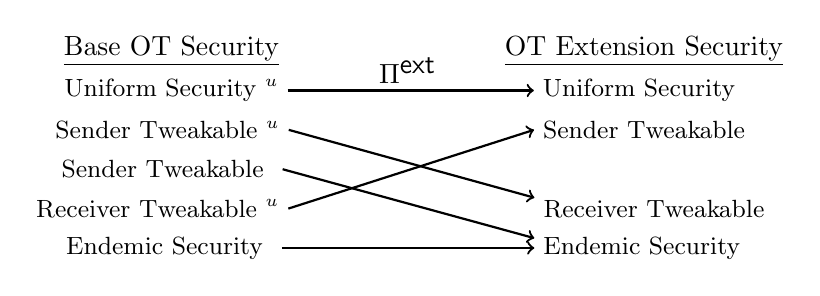
\begin{tikzpicture}[scale=0.5]\small
	\node (pi) at (6,4.5) {\normalsize $\Pi^\textsf{ext}$};
	\node (Base) at (0,5) {\underline{\normalsize Base OT Security}};
	\node (U) at (0,4) {Uniform Security $\OOT^{\U u}$};
	\node (SCu) at (-0.1,3) {Sender Tweakable $\OOT^{\send u}$};
	\node (SC) at (-0.1,2) {Sender Tweakable $\OOT^{\send}$};
	\node (RC) at (-0.35,1) {Receiver Tweakable  $\OOT^{\rec u}$};
	\node (E) at (-0.05,0) {Endemic Security  $\OOT^{\E}$};
	
	
	\node (Ext) at (12,5) {\underline{\normalsize OT Extension Security}};
	\node (EU) at (12,4) {Uniform Security $\OOT^{\U}$};
	\node (ESC) at (12.13,3) {Sender Tweakable $\OOT^{\send}$};
	\node (ERC) at (12.38,1) {Receiver Tweakable  $\OOT^{\rec}$};
	\node (EE) at (12.07,0) {Endemic Security  $\OOT^{\E}$};
%	\draw [-implies,double equal sign distance] (U) -- (SC);
%	\draw [-implies,double equal sign distance] (U) -- (RC);
%	\draw [-implies,double equal sign distance] (SC) -- (E);
%	\draw [-implies,double equal sign distance] (RC) -- (E);
	\draw [->, thick] (U) -- (EU);
	\draw [->, thick] (E) -- (EE);
	\draw [->, thick] (SCu.east) -- (ERC.175);
	\draw [->, thick] (RC.east) -- (ESC.west);
	\draw [->, thick] (SC.east) -- (EE.175);
	
%	\draw [-, thick] (5,2.5)-- (TC);
%	\draw [->, thick] (E) .. controls (1,0.75) .. (SC);
%	\draw [->, thick] (E) .. controls (7,0.75) .. (RC);
	\end{tikzpicture}
	\label{fig:OTExtrelations}
	\caption{
		The figure depicts the implication different Base OT security notions (\definitionref{def:otSec}) have on the result OT extension protocol.  $A\rightarrow B$ denotes that any OT realizing security $A$ can be efficiently transformed by $\Pi^\textsf{ext}$ into an OT extension realizing security $B$, where $\Pi^\textsf{ext}$ is the protocol of \figureref{fig:otExt} such that $\OOT$ is the left hand side oracle.
	}
\end{figure}










Next we review the OT extension protocol of \cite{RSA:OrrOrsSch17} which we describe in \figureref{fig:otExt}. The base OTs are performed on inputs that are sampled uniformly at random where the roles of the sender and receiver are reversed with respect to the OTs that are output by the extension. That is, \send will receiver $(b_j, \tt^j_{b_j})\in\mathbb{F}_2\times \mathbb{F}_2^m$ while $\rec$ will receive $(\tt^j_0,\tt^j_1)\in\mathbb{F}_2^m\times \mathbb{F}_2^m$ for $j\in[\nc]$.

\rec forms two matrices $T_0,T_1\in \mathbb{F}_2^{m\times \nc}$ by concatenating the base OT messages as column vectors, i.e. $T_i:=(\tt^1_i ... \tt^\nc_i)$. Similarly, \send forms the matrix $T_{\text{\textbf{b}}}:=(\tt^1_{b_1}...\tt^\nc_{b_\nc})$. \rec then encodes their 1-out-of-$N$ selections $\ww_1,...,\ww_m$ into a matrix $C\in \mathbb{F}_2^{m\times \nc}$. Each row $\cc_i$ is the codeword $\mathcal{C}(\ww_i)$ of \rec's $i$-th selection $\ww_i\in [N]$, $\mathcal{C}$ is a binary code of length $\nc$, dimension $\kc=\log_2\kappa$ and minimum distance $\dc\geq\kappa$. \rec sends the matrix
$$
	U=T_0+T_1+C
$$
to \send. Observe that $U$ encodes the selections of \rec but the selection is perfectly masked/encrypted due to the $j$-th column of $U$ being masked by the column $\tt^j_{1-b_j}$ which is uniformly distributed in the view of \send. Upon receiving $U$, \send computes $Q\in\mathbb{F}^{m\times\nc}$ where the $j$-th column is defined as $\qq^j:=b_j\cdot \uu^j+\tt^j_{b_j}=b_j\cdot \cc^j+\tt^j_0$. It holds that 
$$
	\qq_i=\cc_i\odot \bb + \tt_i
$$
where $\tt_i,\qq_i$ is the $i$-th row of $T_0,Q$, respectively, and $\bb:=(b_1,...,b_\nc)\in \mathbb{F}^\nc_2$. \rec will output $\vv_{i,\ww_i}:=\H(i, \tt_i)$. \send can then generate any OT message by computing $\vv_{i,\ww}:=\H(i, \qq_i + \mathcal{C}(\ww)\odot \bb)$. Correctness of this operation follows from 
\begin{align*}
	\qq_i + \mathcal{C}(\ww)\odot \bb =&  (\mathcal{C}(\ww_i)\odot \bb + \tt_i) + \mathcal{C}(\ww)\odot \bb\\
	=& (\mathcal{C}(\ww_i) + \mathcal{C}(\ww)) \odot \bb +\tt_i.
\end{align*}
Let $\delta = \mathcal{C}(\ww_i) + \mathcal{C}(\ww)$. In the event that $\ww_i=\ww$, then $\delta=0$ and \send computes the same $\vv_{i,\ww_i}$ value as \rec. Otherwise the hamming distance $\textsf{HD}(\delta)\geq \dc\geq \kappa$ by construction of $\mathcal{C}$. For $\rec$ to generate any other OT message $\vv_{i,\ww}$ s.t. $\ww\neq \ww_i$, \rec must guess the value $\delta\odot \bb\in \mathbb{F}^\nc_2$ given $\delta$, which takes time $2^{\textsf{HD}(\delta)}=O(2^\kappa)$.

To realize the ideal Sender Chosen Message oracle $\OOT^\send$ \cite{C:IKNP03,EC:ALSZ15,C:KelOrsSch15,RSA:OrrOrsSch17} specify two additional steps:
\begin{enumerate}

	\item A proof that all rows in $C$ are valid codewords. Ishai et al. \cite{C:IKNP03} proposed a cut-and-choose approach while the more recent schemes \cite{C:KelOrsSch15,RSA:OrrOrsSch17} improve on the efficiency of these proofs by making \rec send random linear combinations of $\tt_i,\ww_i$ and having \send check they are consistent with same combination of $U$. We defer the details behind these proofs to \cite{C:KelOrsSch15,RSA:OrrOrsSch17} but conclude that these checks (e.g. \stepref{step:consistency} of \figureref{fig:otExt}) ensure that with probability at least $1-\negl$ either $U=T_0+T_1+C$ s.t. $\forall i\in [m] \exists \ww, \cc_i=\mathcal{C}(\ww)$ or \send aborts.
	
	\item The parties apply the Sender Chosen OT transformation $\Pi^{\send}_{1,N}$ from \figureref{fig:protoSendOT} which reduces sender chosen to endemic OT. That is, \send must send their chosen messages $(x_{i,1},...,x_{i,N})_{i\in [m]}$ encrypted under the corresponding key $(\vv_{i,1},...,\vv_{i,N})_{i\in [m]}$, e.g. \send sends $e_{i,j}:=x_{i,j}+\vv_{i,j}$ to \rec who outputs $x_{i,\ww_i}=e_{i,\ww_i}+\vv_{i,\ww_i}$. Note, this step is not included in \figureref{fig:otExt}. Next we will show without this step the protocol only achieves endemic security.
\end{enumerate}




\begin{figure}[t!]
	\vspace{-1cm}
	\framebox{\begin{minipage}{0.95\linewidth}\small
			\textsc{Parameters:} $\kappa$ is the computational security parameter. $m$ denotes the number of OTs. $N$ denotes the number of messages each OT has. $\mathcal{C}$ is an $[\nc,\kc,\dc]$ binary linear code such that $\kc=\log_2 N$ and $\dc\geq \kappa$.\\
			\textsc{Requirements:} $\H : [m] \times \mathbb{F}_2^\nc \rightarrow \mathbb{F}_2^\kappa$ 
			%and $\H' : \mathbb{F}^{(m+\kappa)\times \nc}_2 \rightarrow \mathbb{F}^{m\times \kappa}_2$ are 
			is a random oracle. % and $\PRG : \{0,1\}^{\kappa} \rightarrow \{0,1\}^{m+\kappa}$ is a pseudorandom generator. 
			
			$\O^{\textsf{chllng}} : \mathbb{F}^{(m+s)\times \nc}_2 \rightarrow \mathbb{F}^{m\times s}_2$ is an oracle that returns a challenge string to both parties. Let $m'=m+s$. 	$\OOT$ is an 1-out-of-2 OT oracle with output messages in $\mathbb{F}_2^{m'}$.
			\\
			
			\begin{enumerate}
				\item\label{step:extInit} Both parties invoke $\nc$  instances of $\OOT$  where \send takes the role of the receiver. If $\OOT$ has inputs, the corresponding party  locally samples them uniformly from the input domains. \send receives $(\bb\in\{0,1\}^\nc, \{\tt^j_{b_j}\}_{j\in [\nc]})$. \rec receives $\{(\tt^j_0,\tt^j_1)\}_{j\in [\nc]}$. Let $T_0\in \mathbb{F}^{m'\times \nc}_2$ denote the matrix formed by concatenating the column vectors $\tt^0_0||...||\tt^\nc_0$. \\
				
				%				\item \rec constructs matrices $T_0,T_1\in \mathbb{F}^{m'\times \nc}_2$ from the seeds $\{(\rr^j_0,\rr^j_1)\}_{j\in [\nc]}$ so that the respective columns are:
				%				$$
				%					\tt^j_0 := \PRG(\rr^j_0)\in \mathbb{F}^{m'}_2,\qquad \tt^j_1 := \PRG(\rr^j_1)\in \mathbb{F}^{m'}_2,\qquad \forall j\in[\nc]
				%				$$
				%				In the same way \send produces $\tt^j_{b_j}$, for each $j\in[\nc]$. Summarizing, \rec holds $\{(\tt^j_0,\tt^j_1)\}_{j\in[\nc]}$ and \send holds $\{\tt^j_{b_j}\}_{j\in[\nc]}$.
				%				
				\item\label{step:extSendU} \rec samples random $\ww_{m+\ell}\gets \mathbb{F}^\kc_2$, for $\ell\in[s]$, and then constructs a matrix $C\in\mathbb{F}^{m'\times \nc}_2$ such that each row $\cc_i$ is the codeword $\mathcal{C}(\ww_i)$. Then, \rec sends to \send the values
				$$
				\uu^j :=\tt^j_0 +\tt^j_1+\cc^j, \qquad \forall j\in[\nc],
				$$
				where $\cc^j$ is the $j$-th column of $C$.
				
				\item\label{step:extCompQ} \send receives $\uu^j\in\mathbb{F}^{m'}_2$ and computes
				$$
				\qq^j := b_j \cdot \uu^j +\tt^j_{b_j} = b_j\cdot \cc^j+\tt^j_0,\qquad \forall j\in[\nc]
				$$
				that form the columns of an $(m'\times \nc)$ matrix $Q$. Denoting the rows of $T_0, Q$ by $\tt_i,\qq_i$, \rec now holds $\cc_i,\tt_i$ and \send holds $\bb, \qq_i$ so that 
				$$
				\qq_i = \cc_i\odot \bb+\tt_i,\qquad \forall i\in[m'].
				$$
				
				\item \emph{Consistency check:}\label{step:consistency}
				\begin{itemize}
					\item Both parties query the challenge oracle $\O^{\textsf{chllng}}$ on input $u^j$ for $j\in[\nc]$  which samples and returns $X=\{(x_1^{\ell}, ...,x_m^{\ell} )\in \mathbb{F}^m_2\}_{\ell\in[s]}$ % := H'(\uu^1|| ... || \uu^\nc).
					to both parties.
					
					\item \rec computes and sends, for $\ell \in[s]$:
					$$
					\widehat \tt^{\ell} := \sum_{i\in[m]} \tt_i \cdot x_i^\ell + \tt_{m+\ell}, \qquad \widehat \ww^\ell := \sum_{i\in[m]} \ww_i \cdot x_i^\ell + \ww_{m+\ell}
					$$
					
					\item \send computes $\widehat \qq^\ell := \sum_{i\in[m]} \qq_i \cdot x^\ell_i + \qq_{m+\ell}$, and checks that:
					$$
					\widehat\tt^\ell + \widehat\qq^\ell = \mathcal{C}(\widehat\ww^\ell) \odot \bb, \qquad \forall\ell\in[s].
					$$
					If the check fails, \send sends $\textsf{Abort}$, and otherwise continues.
				\end{itemize}
			\end{enumerate}
			
			\textbf{Output:} \send outputs $\vv_{\ww,i}:=\H(i,\qq_i+\mathcal{C}(\ww)\odot \bb), \forall i\in[m]$ and $\ww\in S_i$. \rec outputs $\vv_{\ww,i}:= \H(i,\tt_i), \forall i\in[m]$.
	\end{minipage}}
	\caption{ 1-out-of-$N$ OT Extension.}
	\label{fig:otExt}
\end{figure}


\begin{figure}[t]
	\framebox{\begin{minipage}{0.95\linewidth}\small
			\textsc{Parameters:} $\lambda$ is the statistical security parameter.
			
			\textbf{Inputs:} \send inputs $U\in\mathbb{F}^{(m+\lambda)\times n}_2$ and \rec inputs $U'$.
			\begin{enumerate}
				\item \send uniformly samples $X\gets \mathbb{F}^{m\times n}_2$ and sends it to \rec.
				\item Both parties output $X$.
			\end{enumerate}
	\end{minipage}}
	\caption{ Challenge Protocol $\Pi^\textsf{chllng}$ implementing $\O^\textsf{chllng}$.}
	\label{fig:OChallenge}
\end{figure}


\subsection{OT Extension Attacks}

The authors of \cite{C:KelOrsSch15,RSA:OrrOrsSch17} provide protocol descriptions that are intended to satisfy the Uniform Message security notion, \definitionref{def:otSec}, but we show this to not be the case. For the rest of this work we will refer to the protocol of \cite{RSA:OrrOrsSch17} as defined in \definitionref{def:OOS} but note that the attacks on Uniform Message security also apply to \cite[Figure 6, 7]{C:KelOrsSch15}. In particular, we detail two attacks where the first (\lemmaref{lem:malSend}) allows a malicious \send to bias the OT messages such that they are all equal while the second attack (\lemmaref{lem:malRec}) allows a malicious \rec to bias the OT messages that they output. In both cases, the ability to bias the messages violates the ideal functionality which samples them uniformly at random.


\begin{definition}\label{def:OOS}
	Let $\Pi^{\textsf{OOS}}$ be the protocol of \figureref{fig:otExt} where $\O^{\textsf{chllng}}:=\Pi^{\textsf{chllng}}$ (\figureref{fig:OChallenge}) and $\OOT:=\OOT^\send$ (\definitionref{def:ot}), i.e.  \cite[Protocol 2]{RSA:OrrOrsSch17}.
\end{definition}
\begin{remark}\label{remark:oosROT}
	\cite{RSA:OrrOrsSch17} is inconsistent which type of base OTs should be used, switching between standard Sender Chosen Message OT ($\OOT^\send=\mathcal{F}^{\kappa,\nc}_{\textsf{2-OT}}$) in the protocol description, theorem statements and Uniform Message OT ($\OOT^\U=\mathcal{F}^{\kappa,\nc}_{\textsf{2-ROT}}$) in their proof. Giving the benefit of the doubt we note that \lemmaref{lem:malRec} would not apply if Uniform Message base OTs are employed as their proofs suggests was their intension. However, the more serious \lemmaref{lem:malSend} attack still applies.
\end{remark}




\lemmaref{lem:malSend} details an attack which performs an extension of size $m=\kappa$ and can distinguish the ideal oracle $\OOT^\U$ and $\Pi^{\textsf{OOS}}$ with probability $1-2^m$. The core idea is that the malicious \send sets the base OT selection bits to be $\mathbf{b}:=(0,...,0)$. As such $\send$ learns the matrix $T_0$ in full. Recall that the output of \rec is defined to be the hash of the rows of $T_0$. Therefore \send can output the same message $\H(i, \tt_i)=\vv_{i,\ww_i}$ as \rec. For Sender Tweakable or Endemic security a viable simulation strategy is to extract $H(i, \tt_i)$ and define $\vv_{i,j}:=\H(i, \tt_i)$ for all $j$. However, there is no valid strategy for the Receiver Tweakable or Uniform Message security where the oracle samples some of the messages uniformly at random.

\begin{lemma} \label{lem:malSend}
	There exists a ppt adversary $\Adv$ and distinguisher $D$ such that for any $\Adv'$ 
	$$
		|\Pr[D((\Adv, \rec)_{\langle\Adv,\rec\rangle})=1]-\Pr[D((\Adv', \O^{\E}_{\textsf{OT,\rec}})_{\langle\Adv',\O^{\E}_{\textsf{OT}}\rangle})=1]|=1-\negl
	$$
	where $\langle\Adv,\rec\rangle$ is the $\Pi^{\textsf{OOS}}$ protocol (\definitionref{def:OOS}), $\O^{\E}_{\textsf{OT,\send}}$ is the \send's side output within the view of $\OOT^{\E}$ and all algorithms additionally receive input $1^\kappa$. 
\end{lemma}
\begin{proof} 
	For simplicity let $N=2$ and $m=\kappa$. We define $\Adv$ as follows. $\Adv$ plays the role of \send and replaces the input to $\OOT^\send$, the receiver input, with the string $\bb:=\{0\}^\nc$. \Adv outputs the matrix $Q$.
	
	We define $D$ as follows. $D$ samples the selection bits $x_1,...,x_m\gets\{0,1\}$ and sends them to \rec. $D$ executes $\Adv$ who outputs $Q$ and \rec outputs $\vv_{x_1,1},...,\vv_{x_m,m}$. If $\vv_{x_i,i}=\H(i,\qq_i)$ for $i\in[m]$, output 1, otherwise 0. In the real interaction it clearly holds that $\Pr[D((\Adv, \rec)_{\langle\Adv,\rec\rangle})=1]=1$ since $\qq_i=\tt_i$.
	
	By definition the input of $\Adv'$ is independent of $x_i$ and receives no output from $\OOT^\E$ (apart from their input $(\vv_{0,i},\vv_{1,i})_{i\in [m]}$). Therefore, it must hold that $\Pr[D((\Adv', \rec)_{\langle\Adv',\O^{\E}_{\textsf{OT,\send}}\rangle})=1]=2^{\kappa}$.
\end{proof}

\lemmaref{lem:malRec} details another attack which allows \R to bias the output $\vv_{i,\ww_i}$ to be $\H(i,x)$ for any $x\in\mathbb{F}^{\nc}_2$. The distinguisher compares the output of \send with $\vv_{i,\ww_i}$ and outputs 1 if they are equal. As \remarkref{remark:oosROT} states, \cite{RSA:OrrOrsSch17} is inconsistent which type of base OTs should be used and this attack only applies if $\OOT^\send=\mathcal{F}^{\kappa,\nc}_{\textsf{2-OT}}$ base OTs are used. This attack does apply to \cite{C:KelOrsSch15}.


\begin{lemma} \label{lem:malRec}
	There exists a ppt adversary $\Adv$ and distinguisher $D$ such that for any $\Adv'$ 
	$$
	|\Pr[D((\send, \Adv)_{\langle\send, \Adv\rangle})=1]-\Pr[D((\O^{\U}_{\textsf{OT,\send}}, \Adv')_{\langle\OOT^\U, \Adv'\rangle})=1]|=1-2^{-\kappa}
	$$
	where $\langle\send, \Adv\rangle$ is the $\Pi^{\textsf{OOS}}$ protocol (\definitionref{def:OOS}), $\O^{\U}_{\textsf{OT,\send}}$ is the \rec's side output within the view of $\OOT^{\U}$ and all algorithms additionally receive input $1^\kappa$. 
\end{lemma}
\begin{proof}
	For simplicity let $N=2$ and $m=1$. We define $\Adv$ as follows. $\Adv$ plays the role of \rec and replaces the input to base OTs, the sender input, with strings $\tt_0^j,\tt_1^j\in \{0\}^{m'}$ and then completes the protocol as normal.
	
	We define $D$ as follows. $D$ executes \send and \Adv with input $x_1=0$. \send outputs $(\vv_{0,1},\vv_{1,1})$ and $D$ outputs 1 if $\vv_{0,1}=\H(1, \{0\}^\nc)$ and 0 otherwise. In the real interaction it clearly holds that $\Pr[D((\send, \Adv)_{\langle\send, \Adv\rangle})=1]=1$. In the ideal interaction the honest \send will output a uniformly distributed $\vv_{0,1}\in\{0,1\}^\kappa$ which was sampled by $\OOT^{\U}$ and therefore $\Pr[D((\send, \Adv')_{\langle\O^{\U}_{\textsf{OT,\rec}}, \Adv'\rangle})=1]=2^{-\kappa}$.
\end{proof}



\subsection{OT Extension Security}


\begin{lemma}
	The $\Pi^\textsf{OOS}$ protocol (\definitionref{def:OOS}) is a 1-out-of-$N$ Oblivious Transfer ($\OOT^\E$) satisfying Endemic Message and Receiver Selection Security (\definitionref{def:otSec}).
\end{lemma}
\begin{proof}
	Correctness of the protocol was demonstrated by \cite{RSA:OrrOrsSch17}. The rest of the proof is essentially the same as \cite{RSA:OrrOrsSch17} except that the simulator extracts the messages from the malicious party.
	\begin{claim}[Malicious Sender Security]
		$\Pi^\textsf{OOS}$ satisfies Security Against a Malicious Sender (\definitionref{def:otSec}) with respect to the $\OOT^\E$ oracle.
	\end{claim}
	\begin{proof}
		Consider the following hybrids which will define the simulator $\Adv'$. 
		\begin{enumerate}[leftmargin=1.8cm]
			\item[Hybrid 1.] $\Adv'$ internally runs \Adv while plays the role of $\rec$ and base OT oracle $\OOT=\OOT^\send$. $\Adv'$ receives $\bb\in \mathbb{F}^\nc_2$ from \Adv in  \stepref{step:extInit} and samples $\tt^j_{i}$ as \rec would. $\Adv'$ sends $(\bb, \{\tt^j_{}\})$ to $\Adv$ on behalf of \OOT. $\Adv'$ outputs whatever \Adv outputs. The view of $\Adv$ is unmodified.
			
			\item[Hybrid 2.] For \stepref{step:extSendU} $\Adv'$ does not sample $\tt^j_{1-\bb_j}$ and instead uniformly samples $U\gets\mathbb{F}^{m'\times \nc}_2$. $\Adv'$ sends $U$ to \Adv and then computes $Q$ as \send would. The view of $\Adv$ is identically distributed. This follows from the fact that $\tt^j_{1-\bb_j}$ is uniformly distributed in the view of \Adv and masks the $j$-th column of $U$ in the previous hybrid. 
			
			\item[Hybrid 3.]\label{hybrid:malSendExtract} For each row $\qq_i$, $\Adv'$ defines the circuit $\mathcal{M}_i:[N]\rightarrow\{0,1\}^\kappa$ such that on input $j\in[N]$ it outputs $\H(i, \qq_i+\bb\odot \mathcal{C}(j))$. $\Adv'$ sends $\mathcal{M}_i$ to the ideal oracle $\OOT^\E$ as the sender's input to the $i$-th OT instance. This change allows the ideal oracle to output the same distribution as the real protocol. The view of $\Adv$ is unmodified.
			
			\item[Hybrid 4.] For \stepref{step:consistency} $\Adv'$ uniformly samples $\widehat{\ww}^{\ell}\gets\mathbb{F}^\kc_2$ and computes $\widehat{\tt}^\ell:=\mathcal{C}(\widehat{\ww}^\ell)\odot\bb+\widehat{\qq}^\ell$.  $\Adv'$ sends $(\widehat{\tt}^\ell,\widehat{\ww}^\ell)_{\ell\in[s]}$ to \Adv. This change is identically distributed to the real protocol. In both cases $\widehat{\ww}^{\ell}$ is uniformly distributed due to $\ww_{m+\ell}$ being uniformly distributed in the view of \Adv. 
			
		\end{enumerate}
		Observe that the final hybrid does not depend on the input of $\rec$ and perfectly simulates the output of the honest party. That is, the ideal oracle will have the honest party output $\vv_{i,\ww_i}=\mathcal{M}_i(\ww_i)=\H(\qq_i+\bb\odot \mathcal{C}(\ww_i))$ as defined in \hybridref{hybrid:malSendExtract}. 
	\end{proof}

	\begin{claim}[Malicious Receiver Security]
	$\Pi^\textsf{OOS}$ satisfies Security Against a Malicious Receiver (\definitionref{def:otSec}) with respect to the $\OOT^\E$ oracle.
	\end{claim}
	\begin{proof}
		
	\end{proof}
\end{proof}





